% Standalone research manuscript. Compile twice with XeLaTeX; no shell escape.
% All figures and references are embedded. No font binaries are distributed.
\documentclass[11pt,letterpaper]{article}
\usepackage[margin=.88in,headheight=16pt]{geometry}
\usepackage{fontspec}
\setmainfont{lmroman10-regular.otf}[BoldFont=lmroman10-bold.otf,ItalicFont=lmroman10-italic.otf,BoldItalicFont=lmroman10-bolditalic.otf]
\setsansfont{DejaVu Sans}[Scale=.88]
\setmonofont{DejaVu Sans Mono}[Scale=.76]
\usepackage{amsmath,amssymb,amsthm,mathtools,microtype}
\usepackage{booktabs,tabularx,longtable,array,xcolor,tikz,graphicx}
\usetikzlibrary{arrows.meta,positioning,calc,fit}
\usepackage{enumitem,fancyhdr,titlesec,needspace,caption,placeins}
\usepackage[most]{tcolorbox}
\usepackage[round,authoryear]{natbib}
\usepackage{xurl,hyperref}
\definecolor{ink}{HTML}{251A3B}
\definecolor{purple}{HTML}{673A96}
\definecolor{gold}{HTML}{AF791B}
\definecolor{teal}{HTML}{267D82}
\definecolor{pale}{HTML}{F5F2FA}
\definecolor{muted}{HTML}{6B6377}
\hypersetup{colorlinks=true,linkcolor=purple,citecolor=purple,urlcolor=purple,
 pdftitle={Out-Design: Creating the Freedom to Transform},pdfauthor={Vincent Boucher},
 pdfsubject={Transformational intelligence, equivalent realizations, released capacity, constructive reconfiguration and SUCCESSOR Omega},
 pdfkeywords={Out-Design, transformational intelligence, representation synthesis, released capacity, design for change, capability construction, SUCCESSOR Omega}}
\urlstyle{same}
\setlength{\parindent}{1.1em}\setlength{\parskip}{.23em}
\setlength{\emergencystretch}{2.3em}\setlength{\tabcolsep}{4.5pt}
\renewcommand{\arraystretch}{1.13}
\widowpenalty=10000\clubpenalty=10000
\setlist{nosep,leftmargin=1.5em,topsep=.4em}
\titleformat{\section}{\large\bfseries\color{ink}}{\thesection}{.65em}{}
\titleformat{\subsection}{\normalsize\bfseries\color{ink}}{\thesubsection}{.65em}{}
\titlespacing*{\section}{0pt}{2.4ex plus .4ex}{1ex}
\titlespacing*{\subsection}{0pt}{1.8ex plus .3ex}{.6ex}
\captionsetup{font=small,labelfont=bf}
\pagestyle{fancy}\fancyhf{}
\fancyhead[L]{\small\sffamily OUT-DESIGN}
\fancyhead[R]{\footnotesize\sffamily TRANSFORMATIONAL INTELLIGENCE}
\fancyfoot[L]{\footnotesize\sffamily Vincent Boucher / MONTREAL.AI}
\fancyfoot[R]{\small\thepage}\renewcommand{\headrulewidth}{.3pt}
\renewcommand{\topfraction}{.94}\renewcommand{\bottomfraction}{.86}
\renewcommand{\textfraction}{.06}\renewcommand{\floatpagefraction}{.82}
\newcolumntype{Y}{>{\raggedright\arraybackslash}X}
\newcolumntype{P}[1]{>{\raggedright\arraybackslash}p{#1}}
\newtheorem{theorem}{Theorem}[section]
\newtheorem{proposition}[theorem]{Proposition}
\newtheorem{corollary}[theorem]{Corollary}
\newtheorem{lemma}[theorem]{Lemma}
\theoremstyle{definition}\newtheorem{definition}[theorem]{Definition}
\theoremstyle{remark}\newtheorem{remark}[theorem]{Remark}
\newcommand{\Out}{\textsf{Out-Design}}
\newcommand{\Om}{\texorpdfstring{SUCCESSOR~$\Omega$}{SUCCESSOR Omega}}
\newcommand{\R}{\mathbb R}\newcommand{\N}{\mathbb N}
\newcommand{\Reach}{\operatorname{Reach}}
\newcommand{\cost}{\operatorname{cost}}
\newtcolorbox{thesis}{colback=pale,colframe=purple,boxrule=.45pt,arc=1mm,
 left=10pt,right=10pt,top=8pt,bottom=8pt,breakable}
\newcommand{\phead}[1]{\Needspace{4\baselineskip}\paragraph{#1}}
\newcommand{\paletteicon}{
\begin{tikzpicture}[x=.23cm,y=.23cm,baseline=-2pt]
 \path[fill=gold!19,draw=gold,line width=.55pt] (0,.2) .. controls (-.6,1.5) and (.1,3) .. (1.5,3.3)
 .. controls (3.2,3.7) and (4.1,2.7) .. (4.1,1.8)
 .. controls (4.1,.8) and (3.1,1.7) .. (2.7,1.1)
 .. controls (2.3,.4) and (3,-.2) .. (2,-.4)
 .. controls (1.1,-.6) and (.3,-.4) .. (0,.2);
 \fill[purple] (.6,1.9) circle (.28);\fill[teal] (1.6,2.6) circle (.28);
 \fill[gold] (2.8,2.5) circle (.28);\fill[purple!50] (.6,.75) circle (.28);
 \fill[white,draw=gold!65,line width=.3pt] (1.9,.5) ellipse (.33 and .42);
\end{tikzpicture}}
\newcommand{\F}{\mathcal F}
\newcommand{\K}{\mathcal K}
\newcommand{\C}{\mathcal C}
\newcommand{\Xor}{\mathop{\bigoplus}}
\begin{document}
\thispagestyle{empty}
\begin{center}
{\small\sffamily\color{purple} MONTREAL.AI\quad /\quad TRANSFORMATIONAL INTELLIGENCE $\infty$}\par
\vspace{1.15em}
{\fontsize{42}{47}\selectfont\bfseries\color{ink} Out-Design\ \paletteicon}\par
\vspace{.7em}
{\Large\bfseries Creating the Freedom\\to Transform}\par
\vspace{.55em}
{\normalsize Design systems that make room for their next capability.}\par
\vspace{1.05em}
{\large Vincent Boucher}\par
MONTREAL.AI, Montr\'eal, Qu\'ebec, Canada\par
\vspace{.45em}{\small 21 October 2026\quad /\quad Revised research manuscript}\par
\end{center}
\vspace{.25em}
\begin{abstract}
A system can have a valid future configuration and no admissible first move toward it. The earlier \emph{Out-Design} constructed external staging access. This revision asks whether a purpose-preserving change of realization can release the needed capacity inside the existing architecture. We develop a \emph{release certificate}: an executable replacement that preserves every required service on independent inputs, fits a declared resource envelope, and frees a resource whose location makes the desired transition reachable. A truth-table compiler constructs a joint Boolean program using established bit-parallel techniques. In the worked model, two programs costing 171 abstract instructions jointly are replaced by a checked 111-instruction realization under a 120-instruction worker limit. Eleven required services remain available on eleven worker slots, while one slot becomes vacant. A derived access criterion and an explicit route then realize all eight required endpoint configurations. Reversing which worker is released preserves the same computational saving but enables none of the seven changed endpoints. A saved capability subsequently supports twelve services on those same eleven workers. Complete-domain program checks, independent occupancy search, phase-by-phase functional audits and negative cases establish the finite results. The contribution is the constructive link from equivalent realization to usable transformation capacity, not a new bitslicing algorithm, a hardware benchmark or a claim of autonomous industrial invention.
\end{abstract}
\begin{thesis}
\centering\large\bfseries
Preserve what the system must do.\\[.25em]
\normalsize Redesign what it can become.
\end{thesis}
\noindent{\small\sffamily THEORY\quad $\cdot$\quad EXECUTABLE CONSTRUCTION\quad $\cdot$\quad CAPABILITY INHERITANCE}
\clearpage

\section{Every worker is occupied. The next move does not exist.}
Eleven required services occupy eleven workers. None may be dropped. A new placement would satisfy the requirements, but every destination is occupied. The permitted relocation moves a service into a compatible empty worker. There is no empty worker. There is no legal first move.

One answer is to acquire another worker. The first edition of \emph{Out-Design} studied exactly that kind of enabling construction: provide a qualified staging resource, and connect it to the places where change is blocked \citep{design1}. This paper asks a different question:

\begin{thesis}
\textbf{Can the system create the room for its own transformation by changing how it fulfills its existing obligations?}
\end{thesis}

The move is not to delete a requirement, wait for a convenient lull, or pretend that a busy worker is empty. It is to construct and qualify another realization of the required functions. In the worked example, two independently requested services can share one worker after their implementations are compiled into a bit-parallel program. Both still produce exactly the required outputs. Their inputs need not agree. Their resource use fits the same worker limits. An existing worker is then released, and its vacancy can make the previously blocked transition possible.

The most important result is not the instruction reduction by itself. The released capacity changes what the architecture can do next. The same saving in the wrong location leaves the intended transformation blocked. A useful design therefore joins three questions: what behavior must remain, how that behavior can be realized differently, and which change the released resource actually enables.

\subsection{From designing an object to designing its next freedom}
An endpoint-oriented designer asks what arrangement performs best now. A change-aware designer also asks how to move between arrangements. A transformational designer can challenge the realization that made those movements impossible in the first place. The output becomes a functioning system with a qualified means of becoming something else.

This is the continuation of our series. \emph{Transformational Intelligence} makes inherited formulations editable while preserving the authorized purpose \citep{ti}. \emph{Out-Evolve} targets capabilities from which later discoveries and constructions can grow \citep{evolve}. \emph{Out-Strategise} constructs useful options and changes when commitments must be made \citep{strategise}. \emph{Out-Execute} makes completed work an executable inheritance \citep{execute}. Here, \emph{Out-Design} constructs a new option by redesigning the means that currently consume the resource it needs.

\begin{thesis}
\textbf{A design can do more than survive change. It can help make the next useful change possible.}\\[.25em]
The capability to transform is part of what the design delivers.
\end{thesis}

\subsection{The boundary we deliberately change}
The original model preserves \emph{distinct components}, each at one compatible location. The new digital model preserves \emph{distinct service contracts}, while permitting their code to be realized jointly. These are different invariants. A unique physical specimen, a mandated separate implementation, or an isolation requirement cannot be replaced by a shared program merely because their output tables look alike.

Our new construction applies only where the purpose actually permits implementation replacement and joint execution. It does not refute the earlier theorem that a fully occupied fixed-token architecture needs a vacancy. It constructs a state outside that fixed-realization model while preserving the explicit service requirement in the new setting: every named function, on every admitted independent input, within its declared operating envelope.

\subsection{The developed contribution}
Bit-parallel implementation, consolidation, program transformation and matching reconfiguration are established techniques \citep{biham,usuba,ferdaus,aichholzer}. The scientific contribution here is their explicit constructive coupling: a checked program releases a particular occupied resource; a necessary-and-sufficient access condition says whether that release enables the requested endpoint; a route realizes it; and a successor uses the saved release capability to add a genuinely new function. Each link is represented and executed rather than supplied as an unverified label.

This is a finite research construction, not a claim that a new universal design algorithm has been discovered. The compiler searches two stated representation forms. A capable specialist given the same compiler can obtain the same result. The ambitious object is nevertheless precise: \emph{an architecture whose existing functions can be reorganized to make a new capability possible without adding a worker}.

\section{The complete demonstration in one view}
\label{sec:overview}
The worked system contains three groups of three services, plus a required donor service $r$ and a required host service $h$. Every service initially has a worker. Within each three-service group, compatibility permits the identity placement or one cyclic permutation. The donor and host must return to their original positions at every terminal reconfiguration. There are therefore eight required terminal placements, with the same eleven functions throughout.

A designated member of each group may temporarily occupy the donor's worker. That ordinary compatibility is useful only if the worker can be vacated. The host can execute an admitted replacement program, subject to unchanged limits: 120 bitwise instructions per batch, 144 conservative scratch words, twelve input words, and two code banks with at most 240 instruction records in total. These are explicit abstract-machine limits, not hardware timings.

The compiler receives complete truth tables for $r$ and $h$. Their separately emitted programs require 86 and 85 instructions. Running those programs sequentially on one worker would require 171 and violate the 120-instruction limit. A joint representation requires 111, including twelve packing instructions and three output-decoding instructions. It uses 123 conservative scratch words. Its complete $64\times64$ independent-input domain is checked.

\begin{figure}[htbp]\centering
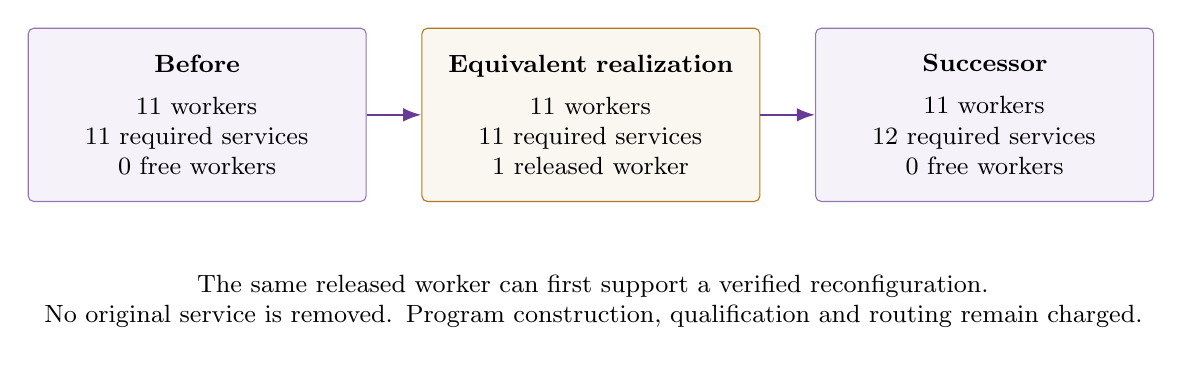
\begin{tikzpicture}[font=\small,>=Latex,
 box/.style={draw=purple!70,fill=pale,rounded corners=2pt,align=center,text width=3.8cm,minimum height=2.2cm,inner sep=7pt}]
\node[box] (a) at (0,0) {\textbf{Before}\\[.45em]11 workers\\11 required services\\0 free workers};
\node[box,draw=gold,fill=gold!6] (b) at (5.0,0) {\textbf{Equivalent realization}\\[.45em]11 workers\\11 required services\\1 released worker};
\node[box] (c) at (10.0,0) {\textbf{Successor}\\[.45em]11 workers\\12 required services\\0 free workers};
\draw[->,thick,draw=purple] (a)--(b);
\draw[->,thick,draw=purple] (b)--(c);
\node[below=8mm of b.south,align=center,text width=14cm] {The same released worker can first support a verified reconfiguration.\\No original service is removed. Program construction, qualification and routing remain charged.};
\end{tikzpicture}
\caption{Executed digital construction. Counts refer to the declared local worker model, not physical servers or a claim of distributed uptime. Resource limits remain unchanged; the implementation uses previously unexploited word-parallel capacity and admitted memory.}
\label{fig:headline}
\end{figure}

Once the joint realization is active at $h$, $r$'s worker can be retired as a separate realization. The required service $r$ remains active through the host. The empty worker then serves as the intermediate location for rearranging the groups. Twelve checked relocations perform all three cycles. Restoring the separate donor realization returns the system to its required terminal shape.

A later mission chooses a different use for the same release. It keeps the qualified joint realization and installs a new threshold function in the released worker. The number of required services rises from eleven to twelve, on the same eleven worker slots. The new function is not a renamed old service, and its program and qualification are added to the account.

\begin{table}[htbp]\centering\small
\caption{The decisive distinction in the worked model. A resource saving is not yet a transition capability. Both ordered joint realizations have identical instruction counts.}
\begin{tabularx}{\linewidth}{@{}Yrr@{}}\toprule
Realization choice & Joint instructions & Reachable required endpoints\\\midrule
No joint realization; no extra worker & --- & 1 of 8\\
Joint program at $r$, releasing $h$ & 111 & 1 of 8\\
Joint program at $h$, releasing $r$ & 111 & \textbf{8 of 8}\\\bottomrule
\end{tabularx}
\label{tab:direction}
\end{table}

This is why the paper is about design rather than only code optimization. Releasing the host's worker produces exactly as much empty capacity, but the group services cannot reach it. The constructor must select \emph{where the representation change takes place} according to the transformation it is meant to enable.

\section{Keep the function fixed; make its realization editable}
\label{sec:model}
\subsection{A service contract with a complete finite meaning}
Let the required services be $\F=\{f_i:i\in V\}$, with each
\begin{equation}
 f_i:\{0,1\}^{w}\longrightarrow\{0,1\}.
 \label{eq:services}
\end{equation}
A batch supplies one independent $w$-bit vector $x^{(i)}$ to every service. The required response is the full indexed vector $(f_i(x^{(i)}))_{i\in V}$. Inputs are not assumed equal, synchronized in value, or statistically related. Their batch boundary is a control assumption, not an equality assumption.

An implementation partitions service identities among active worker kernels. A kernel assigned identities $J$ must return their individual outputs for every element of the Cartesian product of their input domains. A single kernel may cover several services only after that complete contract is established. Counting one function twice does not fulfill two distinct functions; dropping an inconvenient input does not qualify a replacement.

A worker's resource envelope is
\begin{equation}
 B=(L,M,I,C,W),
 \label{eq:budget}
\end{equation}
where $L$ bounds straight-line instruction count per batch, $M$ bounds conservative live storage, $I$ bounds input registers, $C$ bounds the two resident code banks, and $W$ is word width. This is a vector of different resource constraints. We do not sum them into a fictitious intelligence score.

The worked values are $(120,144,12,240,64)$. The instruction set is fixed-width AND, XOR, and shifts by admitted constant amounts. Integer immediates are encoded operands. Each emitted operation costs one abstract instruction. There are no table-lookup, conditional, whole-function or uncharged vector-evaluation instructions in this grammar. A more capable machine with a cheap lookup primitive can have a better implementation and must be compared on its actual terms.

\subsection{A release certificate}
\begin{definition}[Qualified release]
A release certificate for an ordered donor--host pair $(r,h)$ contains: their complete source contracts; an executable joint kernel $K_{rh}$; a proof or exhaustive check that
\begin{equation}
 K_{rh}(x,y)=(f_r(x),f_h(y))\qquad\text{for every independent }(x,y);
 \label{eq:fusion}
\end{equation}
a resource account satisfying $B$; a permitted batch-boundary promotion that transfers the two active service identities to $h$; and the procedure for retiring or restoring the separate donor realization. It also names the original worker that becomes vacant.
\end{definition}

The certificate is more than a smaller program. It connects an equivalent realization to a usable architectural change. Promotion must preserve every other service and must not exceed the preparation code-bank allowance. A downstream route must respect the compatibility and capacity conditions of the newly vacant worker.

\begin{proposition}[Functional release under a preserved envelope]
\label{prop:release}
Suppose a checked joint kernel satisfies Equation~\eqref{eq:fusion}, fits the host's unchanged resource envelope, and can be promoted atomically between batches while every other kernel is unchanged. Retiring the donor's separate active realization preserves the complete service output for every admitted batch and releases one existing worker. No additional worker is required by this operation. Restoring the two individually qualified realizations reverses it.
\end{proposition}
\begin{proof}
Every unaffected output remains the output of its unchanged kernel. The two replaced outputs agree with their original contracts by Equation~\eqref{eq:fusion} on the complete product input domain. The active service map contains each identity once before and after promotion. All resident and active programs fit the stated bounds. Retiring the now-inactive donor implementation leaves its worker vacant without removing its service. The same equality supports the reverse replacement.
\end{proof}

The proposition does not produce physical capacity from nothing. The joint program exploits word-level parallelism and memory already admitted by the machine contract. Compiler work, qualification, changed routing, extra input traffic at the host, preparation storage and any real handover costs remain necessary. At the machine level the resource was occupied by a particular realization, not proven irreducibly consumed by its function.

\subsection{When replacement is not permitted}
Some purposes require separate trust domains, independent failures, a unique object, private memory separation or a particular physical implementation. Pointwise output equality does not preserve those properties. They must either enter the contract and its checker or forbid the release. The present emulator makes no claim about timing side channels, mutable distributed state or a physical instrument's continuous output during transport.

This distinction is essential to transformational intelligence. The original purpose is the reference. An implementation choice is editable only when changing it does not erase an actual requirement.

\section{Constructing the joint realization from complete behavior}
\label{sec:compiler}
\subsection{A known representation, made into an executable design primitive}
Bit slicing treats positions within a word as independent Boolean lanes. It is established implementation technology; automated compiler work such as Usuba already systematizes it \citep{biham,usuba}. Our contribution is not the technique itself. It is the checked use of a constructed representation to release a resource selected by an architectural reachability requirement.

Every $w$-input Boolean function has a unique algebraic normal form over $\mathrm{GF}(2)$:
\begin{equation}
 f_j(x)=\Xor_{S\subseteq[w]} a_{j,S}\prod_{k\in S}x_k,
 \qquad a_{j,S}\in\{0,1\}.
 \label{eq:anf}
\end{equation}
The compiler obtains the coefficients from the complete truth table by Boolean-lattice inversion. This is exact finite conversion, not learning from samples. It does not claim that the resulting circuit is the smallest possible implementation of the function.

For $q\le W$ possibly different functions on independent inputs, pack the $k$th input bit of each function into
\begin{equation}
 X_k=\sum_{j=0}^{q-1}2^j x^{(j)}_k,\qquad
 C_S=\sum_{j=0}^{q-1}2^j a_{j,S}.
 \label{eq:packing}
\end{equation}
The emitted word expression is
\begin{equation}
 Y=\Xor_{S\subseteq[w]}\left(C_S\ \mathbin{\&}\ \mathop{\bigwedge}_{k\in S}X_k\right),
 \label{eq:packed}
\end{equation}
with the empty conjunction equal to the active-lane mask $2^q-1$. Zero coefficient masks are omitted. A mask containing every active lane needs no extra AND. The constant term is an immediate. Finally, the program extracts bit $j$ of $Y$ as output $j$.

\begin{theorem}[Independent-input correctness of the emitted program]
\label{thm:packing}
For every complete input tuple $(x^{(0)},\ldots,x^{(q-1)})$, bit $j$ of Equation~\eqref{eq:packed} equals $f_j(x^{(j)})$. The packing and extraction use only fixed-width operations within $W$ when $q\le W$.
\end{theorem}
\begin{proof}
Bitwise AND and XOR act independently at each bit position. At bit $j$, $C_S$ contributes $a_{j,S}$ and the conjunction contributes $\prod_{k\in S}x^{(j)}_k$. The XOR therefore equals Equation~\eqref{eq:anf} for function $j$ on its own input. Packing shifts each Boolean input by its lane index, so distinct inputs occupy disjoint positions and no arithmetic carry is used. Every admitted lane lies below $W$; extraction recovers its Boolean result.
\end{proof}

The functions need not be identical. Their coefficient masks can differ. What is shared is the word-level evaluation of a monomial across independent inputs, not an assumption that two customers asked the same question. A mutation that packs the donor's input into both lanes fails the independent verifier on the explicit input pair $(0,1)$ in our worked case.

\subsection{Every operation that creates the representation is counted}
The compiler emits a straight-line instruction list with explicit operands. For two six-bit services, packing costs twelve instructions: six shifts and six XORs. Extraction costs three: one right shift and two masks. Shared monomials are built through a deterministic prefix recurrence, with one AND for each additional required nontrivial monomial. Lane-specific coefficients add masks where needed. The output is assembled by XOR.

The worked emitted program has six left shifts, 51 XORs, 53 ANDs and one right shift: exactly 111 instructions. Its twelve input registers plus 111 immutable intermediate registers give the conservative 123-word storage account. We do not assume optimal register allocation. The maximum resident host code during preparation is 196 instruction records: its old 85-instruction program plus the 111-instruction replacement, below the 240-record allowance.

\begin{table}[htbp]\centering\small
\caption{Actual emitted programs for the worked pair. These are abstract-machine counts, not processor cycles, wall-clock latency, energy measurements or globally minimum Boolean-circuit sizes.}
\begin{tabularx}{\linewidth}{@{}Yrr@{}}\toprule
Resource & Serial realization & Joint realization\\\midrule
Independent services supplied & 2 & 2\\
Required input words & 12 & 12\\
Emitted instructions & 171 & 111\\
Conservative scratch words & 183 & 123\\
Fits a 120-instruction, 144-word worker & No & Yes\\
Complete independent input combinations & 4096 & 4096\\\bottomrule
\end{tabularx}
\label{tab:program}
\end{table}

The existing scalar compiler and the packed compiler are both available to the design procedure. On some functions serial code is better. A specialized Boolean optimizer, a native vector compiler or a lookup-capable device may do better than either. Those alternatives would expand the implementation grammar; they are not excluded in order to claim universal superiority.

\subsection{A semantic checker distinct from the constructor}
A separate interpreter evaluates the serialized program on every admitted input combination and compares its outputs with direct truth-table lookup. It does not call the compiler's algebraic transform or execution routine. It also rejects forward references, malformed output maps, invalid word widths, unsupported operations and falsified cost summaries. Static resource limits and full-domain correctness are separate qualification results: a correct program can be too expensive to use.

Both implementations were written in the same authoring process. Their agreement is software evidence, not external peer review or a proof-assistant formalization. The algebraic argument and explicit negative cases provide additional, differently structured checks.

\section{Released capacity must be in the right place}
\label{sec:topology}
\subsection{The post-release movement problem}
Let $A_{ij}=1$ mean that singleton service $i$ is qualified at worker $j$. Initially service $i$ occupies $i$ and $A_{ii}=1$. Consider a release of donor $r$ into host $h$. During the transition, $h$ is locked as the joint realization and $r$'s worker is empty. The movable services are
\begin{equation}
 M=V\setminus\{r,h\}.
\end{equation}
A target $\sigma$ is a qualified ordinary permutation that fixes $r$ and $h$. Its nonanchor services must eventually occupy their specified compatible workers. The joint realization is then undone. This is the stated single-release protocol, not every possible sequence of nested fusions.

Construct a directed graph on $M\cup\{r\}$. For $i\in M$, include $i\to j$ when $A_{ij}=1$ and $j\in M\cup\{r\}$. The node $r$ is a vacancy destination, not a movable service; $h$ is unavailable throughout. Define
\begin{equation}
 R_{r\mid h}=\{i\in M:\text{there is a directed path from }i\text{ to }r\}.
 \label{eq:access}
\end{equation}

\begin{theorem}[Exact reachability after qualified release]
\label{thm:reach}
Under the one-vacancy relocation rules and the qualified release above, a compatible terminal permutation $\sigma$ fixing $r,h$ is reachable exactly when
\begin{equation}
 \boxed{\qquad \sigma(i)=i\quad\text{for all }i\in M\setminus R_{r\mid h}.\qquad}
 \label{eq:criterion}
\end{equation}
Every required function remains supplied throughout a route constructed with the admitted batch-boundary handovers. A compiler can decide the condition without enumerating all placements and can construct a route whenever it holds.
\end{theorem}
\begin{proof}
After release, remove the locked host and the donor's separate realization from the movement problem. There are $|M|$ movable singleton realizations and $|M|+1$ available workers. The donor's worker acts as the one empty location. Its qualified direct users are $S_r=\{i\in M:A_{ir}=1\}$.

This is the earlier one-vacancy model on the remaining ordinary compatibility graph, with staging access $S_r$. Its directed access set consists exactly of services that can reach $r$, namely $R_{r\mid h}$. The fixed-token reachability theorem therefore gives Equation~\eqref{eq:criterion} \citep{design1}. For completeness, Appendix~\ref{app:reach} supplies the vacancy invariant and constructive cycle procedure. Proposition~\ref{prop:release} preserves the two anchor services; every ordinary handover preserves its singleton service. Restoring the donor after the vacancy returns to $r$ completes the specified terminal configuration.
\end{proof}

This is a precise reduction to established reconfiguration structure, not a new general matching theorem. Its new design use is that the vacancy is \emph{constructed by equivalent execution}, rather than assumed to be an additional physical slot.

\subsection{Two equally good kernels can create different futures}
The worked family contains escape interfaces from one service in each three-cycle to worker $r$. The host has no corresponding incoming escape. Fusing the pair at $h$ releases $r$ and makes every cycle movable. Fusing the same pair at $r$ releases $h$, locks the useful intermediate location, and changes none of the cycle endpoints that can be reached.

The programs have the same 111-instruction cost and the same correct outputs. One architectural use reaches all eight requested endpoints; the other reaches only the unchanged endpoint. Complete state-space search independently confirms both. Optimization of the kernel alone cannot select the useful design from this tie.

\begin{thesis}
\textbf{Do not optimize a saving in isolation. Design what the saving makes possible.}\\[.25em]
A released resource becomes an enabling capability only when the next construction can actually use it.
\end{thesis}

\subsection{A joint change that neither half achieves alone}
The four-way control preserves the same functions, workers and eight target placements. Without equivalent cohosting, every worker is occupied, so ordinary relocation cannot start. Without escape access, the released donor worker cannot receive a member of any cycle. With both changes, all three cycles can turn.

\begin{table}[htbp]\centering\small
\caption{Exact factorial control. Adding either ingredient alone leaves only the identity endpoint reachable; the joint construction enables all eight. The full-access specialist can construct the same design.}
\begin{tabularx}{\linewidth}{@{}Ycc@{}}\toprule
 & No escape interfaces & Qualified escape interfaces\\\midrule
Fixed separate realizations & 1 & 1\\
Qualified joint realization & 1 & \textbf{8}\\\bottomrule
\end{tabularx}
\label{tab:factorial}
\end{table}

The fusion-only arm is checked by explicit occupancy search. The fixed-realization arms have no empty destination and hence no outgoing legal move. The joint arm has actual checked traces, not merely an enlarged diagram. This is an elementary but exact complementarity: one change supplies capacity; the other makes that capacity usable for the authorized objective.

\section{The constructor returns a capability and a route}
\label{sec:algorithm}
A candidate is not only a program or a layout. It is an ordered release pair, a checked realization, the access architecture, an attaining transition, and a rule for restoration or further use. The implemented pass is deliberately finite and transparent.

\begin{table}[htbp]\centering\small
\caption{The constructed object and its evidence. The functions, budgets, compatibility grammar and permitted promotions are research inputs. Implementations, resource counts, release choice and routes are computed.}
\begin{tabularx}{\linewidth}{@{}P{.16\linewidth}Y@{}}\toprule
Step & Required construction\\\midrule
Specify & Retain all original service contracts, placement obligations and resource limits. Identify which internal realizations may change.\\
Compile & Construct serial and packed candidates from complete behavior. Count packing, arithmetic, output decoding and conservative storage.\\
Qualify & Check every independent input combination; reject semantic or resource failures. Check the preparation envelope as well as steady operation.\\
Locate & For each admitted ordered release, compute which blocked groups can use the resulting vacancy.\\
Realize & Construct the path and independently verify each source, destination, compatibility and preserved function.\\
Retain & Save the executable kernel, scope, resource envelope, architecture and evidence. Recheck inherited identities before a successor uses them.\\\bottomrule
\end{tabularx}
\label{tab:constructor}
\end{table}

The worked selector evaluates both orders of the anchor pair, rather than accepting the first computationally valid fusion. It chooses a budget-qualified candidate that covers the complete target family. A broader search could consider more pairs, more representations or several successive releases. Those policy classes are not silently attributed to this implementation.

The route generator rotates a target cycle through a shortest current access path to the vacancy, then restores any external path members. It recomputes paths using current placements. It is a completeness construction, not a general shortest-path solver. The independent breadth-first reference sometimes finds fewer moves, and those cases remain in the evidence.

\subsection{A release can also be the wrong investment}
A new program might release an irrelevant worker, require too much preparation memory, or create a single point of dependence. Its qualification may cost more than renting a spare worker. Its host may not meet the real latency or isolation obligation. The design procedure must retain those possibilities rather than reward every transformation simply for being different.

In the worked model, a one-instruction tightening below the 111-instruction implementation rejects that implementation. A 122-word scratch limit likewise rejects its 123-word account. These are failures of the named emitted program, not proofs that no better compiler or representation exists.

\section{Execution: every service remains present at every checked phase}
\label{sec:emulator}
The local emulator implements workers with two code banks and one active kernel. Each active service identity has exactly one route. A batch is evaluated under one committed active map. Promotion is atomic between batches. There is no claim that Python implements a real-time scheduler, a distributed transaction, a stateful migration or fault-tolerant network routing.

The fusion phase prepares the joint program in the host's inactive code bank while the old host and donor programs remain active. Qualification precedes promotion. A promotion switches both service identities to the checked joint kernel; the now-inactive donor image is then retired and its worker becomes free. The old host image remains available within the stated code-bank envelope for restoration.

Every ordinary relocation prepares a compatible destination, qualifies it, changes the active route at a batch boundary, and releases the old location. Source and destination code may coexist during preparation, but they occupy only the existing workers and admitted banks. Restoration prepares the donor's separate image, promotes the original pair of kernels, and retires the joint image.

\begin{figure}[htbp]\centering
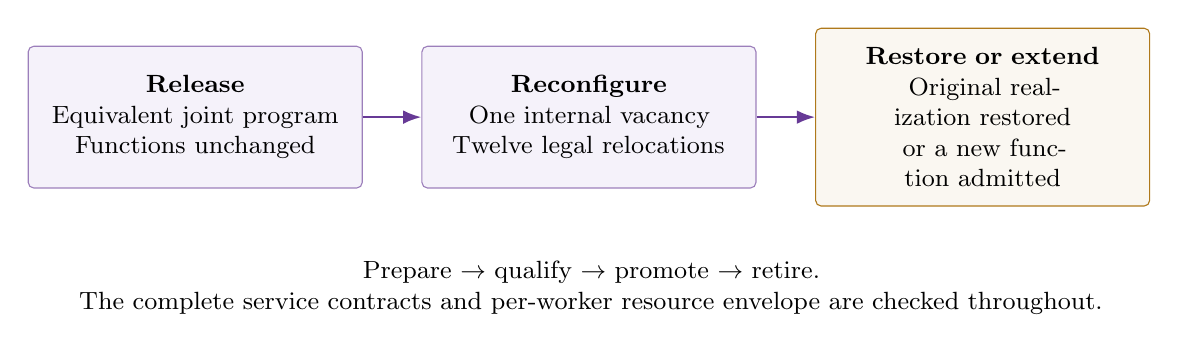
\begin{tikzpicture}[font=\small,>=Latex,
 box/.style={draw=purple!65,fill=pale,rounded corners=2pt,text width=3.75cm,align=center,minimum height=1.8cm,inner sep=7pt}]
\node[box] (a) at (0,0) {\textbf{Release}\\Equivalent joint program\\Functions unchanged};
\node[box] (b) at (5,0) {\textbf{Reconfigure}\\One internal vacancy\\Twelve legal relocations};
\node[box,draw=gold,fill=gold!6] (c) at (10,0) {\textbf{Restore or extend}\\Original realization restored\\or a new function admitted};
\draw[->,thick,draw=purple] (a)--(b);\draw[->,thick,draw=purple] (b)--(c);
\node[below=8mm of b.south,align=center,text width=14cm] {Prepare $\rightarrow$ qualify $\rightarrow$ promote $\rightarrow$ retire.\\The complete service contracts and per-worker resource envelope are checked throughout.};
\end{tikzpicture}
\caption{The executed local transition. All preparation and promotion stages are recorded. The guarantee concerns complete finite functions at the declared batch boundaries, not physical or distributed uptime.}
\label{fig:trace}
\end{figure}

The main trace comprises one initial audit, four fusion-phase audits, four audits for each of twelve relocations, and four restoration audits: 57 states. At every state, the emulator checks all input combinations of each active kernel against the source tables. Single-service kernels have 64 cases; a joint kernel has 4096 independent-input pairs. Across the trace this gives 246,464 kernel-input cases and 459,456 individual output comparisons. Different kernels can be checked separately because their input/output contracts are independent and the router is checked to contain every required identity exactly once.

The maximum active kernel remains at 111 instructions and 123 conservative scratch words. The maximum resident code at one worker is 196 records. No state occupies more than the eleven available worker slots. Quiescent states before and after each primitive also satisfy the movement model's placement requirements.

Compilation and exhaustive qualification occur outside the 120-instruction service-batch account and are explicitly retained as work. The experiment does not demonstrate that they can run concurrently with live requests without affecting latency. It demonstrates correct, resource-checked batch states and permitted transitions in a controlled local model. Real operation needs its own scheduling and handover evidence.

\section{Executed evidence, including where the construction loses}
\label{sec:evidence}
\subsection{Complete-input qualification of fresh program pairs}
The program block contains 64 separately seeded pairs of six-input Boolean functions. Half have related algebraic supports; half are independently generated truth tables. Both serial and packed forms are constructed and tested on all 4096 independent input pairs. All 128 emitted programs agree with their complete source contracts: 524,288 deterministic program--input comparisons.

The resource outcome is selective. Thirty-one fixtures qualify only in packed form, one qualifies only in serial form, one qualifies in both, and 31 qualify in neither under the unchanged 120-instruction and 144-word envelope. Packed code uses fewer instructions in forty fixtures, not all sixty-four. These counts describe the supplied generator, not the prevalence of useful transformations in industry.

\begin{table}[htbp]\centering\small
\caption{Fresh compiler fixtures. Complete-domain correctness and feasibility under the named resource limit are different claims. A rejected pair may admit another implementation outside the two-form grammar.}
\begin{tabularx}{\linewidth}{@{}Yr@{}}\toprule
Recorded quantity & Result\\\midrule
Generated function pairs & 64\\
Complete-domain checks of both emitted forms & 524,288\\
Correct programs & 128/128\\
Only packed form fits & 31\\
Only serial form fits & 1\\
Both forms fit & 1\\
Neither form fits & 31\\
Packed form has strictly fewer emitted instructions & 40/64\\\bottomrule
\end{tabularx}
\label{tab:programstudy}
\end{table}

No language model discovers the primitive instruction set during this study. The truth tables, resource model and representation grammar are authored inputs. The program construction is executed; a general skill for discovering new representations is not established by that execution.

\subsection{A topology reference that does not use the theorem}
The topology study enumerates every directed compatibility matrix on three movable services, a fixed donor and a locked host, allowing all ordinary arcs among the movable services and all arcs from them to the donor vacancy. There are nine optional arcs and $2^9=512$ matrices. Every compatible terminal target is checked.

A separate occupancy implementation performs breadth-first search over actual placements. It imports neither the access-set predictor nor the route constructor. All 1024 feasible target comparisons agree with the criterion. A separate 64-seed block uses six movable services, producing 1512 additional feasible-target comparisons. The complete 2536 comparisons agree.

\begin{table}[htbp]\centering\small
\caption{New release-topology evidence. The original paper's larger static-staging audit is separately reproduced, not merged into these counts.}
\begin{tabularx}{\linewidth}{@{}Yrr@{}}\toprule
Quantity & Exhaustive block & Confirmation block\\\midrule
Compatibility matrices & 512 & 64\\
Feasible target comparisons & 1024 & 1512\\
Oracle occupancy states, summed over matrices & 3048 & 8956\\
Constructed reachable-target paths & 948 & 1500\\
Checked ordinary relocations & 1492 & 8563\\
Constructed paths longer than shortest reference & 0 & 161\\
Maximum excess relocation count & 0 & 8\\\bottomrule
\end{tabularx}
\label{tab:topology}
\end{table}

The route generator is valid on every returned path. It is not shortest on 161 confirmation targets. The main twelve-move route is independently shortest in its specific three-cycle topology, but that does not establish optimality of every generated route. The unfiltered matrices include unreachable targets and harmless identity cases; universal failure is not concealed by discarding them.

\subsection{What the comparisons establish}
A fixed-realization, full-occupancy system cannot begin a nontrivial relocation. The serial pair implementation does not fit the worked host envelope. The packed program does. An additional staging worker can also enable the inherited relay construction, and a sufficiently capable specialist with bit-parallel compilation can reproduce the same internal release.

These are mechanism comparisons. They do not establish superiority over Usuba, a native compiler, an unrestricted synthesis engine or every consolidation policy. The target quantity is a newly exhibited resource-feasible transition in the declared design space. The programs' instruction counts are not wall-clock speedups.

\subsection{Rejection is part of the artifact}
The negative cases include corrupted independent-input packing, insufficient instruction allowance, insufficient scratch storage, missing ordinary escape access, release of the wrong worker, invalid current placement, an unregistered joint kernel, wrong source contracts, occupied destinations and inadequate preparation memory. The new 38-method test suite passes. Every stated rejection is connected to a real condition checked in code; the paper does not infer generic safety from the number of tests.

The original package is preserved byte-for-byte. Its seven deterministic result records reproduce exactly and its 36 test methods pass again. Its 372,800 static-staging target--adapter comparisons, relay access costs and 97-to-121-component family remain results of the earlier model. They are not renamed as additional independent trials of the new representation construction.

\section{The successor adds a function, not just another arrangement}
\label{sec:successor}
Rearranging the same services demonstrates transition capacity. A stronger use of the release is to deliver an additional service. The study therefore writes the accepted capability to disk, reopens that exact record, and uses its retained joint program in a new mission.

The new requirement is a six-input threshold function that returns one exactly when at least four input bits are one. Its truth table differs from every old service table. Its independent request is additional to the eleven original requests. The constructor emits and qualifies a 45-instruction implementation; it does not count the new function as free because a worker can be released.

The retained joint program is requalified on all 4096 pair inputs. It is not synthesized again. After it releases the donor worker, the new program is prepared and qualified there. The new requirement becomes active at the same boundary as its admitted implementation. All eleven original functions remain active, with unchanged semantics. The terminal system supplies twelve distinct service identities on eleven workers.

\begin{table}[htbp]\centering\small
\caption{Actual successor construction. The unchanged resource envelope includes the newly used input lanes and program memory. Full qualification and the new program remain charged.}
\begin{tabularx}{\linewidth}{@{}Yrr@{}}\toprule
Quantity & Predecessor & Successor\\\midrule
Worker slots & 11 & 11\\
Required service identities & 11 & 12\\
Newly supplied threshold service & Absent & Present\\
Original donor/host service instructions, in total & 171 & 111\\
New service instructions & --- & 45\\
Maximum permitted instructions per worker & 120 & 120\\
Instructions for the affected service set & 171 & 156\\
Retained joint program synthesized again & --- & 0 times\\\bottomrule
\end{tabularx}
\label{tab:successor}
\end{table}

The affected services use fifteen fewer abstract instructions per batch even after the new function is included. This is a precise consequence of the emitted programs, not a claim of lower total runtime or energy. The new request contributes six additional input bits to the system; the host accepts twelve input words instead of six, within its pre-existing allowance. The compiler, checker and routing requirements remain separate resources.

The successor trace contains nine audits and 46,720 individual output comparisons. It returns a functioning additional finite service in the model, not a new physical research instrument or an independently funded business. Its significance for \Om{} is the inheritance pattern: an accepted realization can supply the capacity in which a different accepted function is constructed.

\begin{thesis}
\textbf{The saved asset is not an empty slot. It is a verified way to make a slot available when a new capability needs it.}
\end{thesis}

Keeping the joint program permanently changes the successor's failure exposure. Two functions now depend on one host. The original restoration path is no longer available while its worker contains the new service. A rollback, host-failure guarantee, isolation requirement or simultaneous demand outside the batch contract would require additional design. Adding capability does not erase those obligations.

\section{Design for the next attainable capability, not a larger diagram}
\label{sec:scope}
The experiment is computational, but the question it makes concrete is a general design question: which part of the apparent resource shortage is imposed by the present realization, and which part is an actual limit of the authorized purpose?

In a scientific platform, a new measurement interface might replace repeated separate observations with one qualified shared acquisition. In a production system, a reusable fixture might make existing machine capacity accessible to a different operation. In a software-backed instrument, a new representation might release compute or memory needed for an additional analysis. These are prospective domains, not results established by the Boolean laboratory. Each needs a domain-specific equivalence, resource account and safe transition primitive.

The crucial distinction is between \emph{consolidating assumed loads} and \emph{constructing a realization with a different verified load}. Ordinary consolidation can exploit idle resources; it must not assume that two individually expensive services fit because their names look similar. Here the compiler supplies the changed resource profile and the checker establishes the retained semantics. The architecture then determines whether that profile creates a useful next move.

A mature design engine would search several representations and several resource locations together, retain a Pareto set of qualified constructions, and investigate which ones unlock independently specified future requirements. A larger candidate catalogue is not itself evidence of improved discovery. That claim would require campaigns in which a new design process repeatedly constructs better capabilities from comparable initial resources.

\subsection{One principled stop condition}
When no candidate passes, the responsible output is the remaining obstruction. A false function equivalence calls for another implementation. A resource violation calls for a cheaper realization, a larger permitted budget or a different host. A disconnected vacancy calls for a qualified interface or another release location. A forbidden intermediate state calls for another purpose-preserving transition, not a relabeled success.

The compiler's finite grammar can be exhausted without exhausting the design space of science. Conversely, a proposed new primitive does not become valid because it would solve the obstruction. Construction and qualification must earn its semantics and resource claims before the route can rely on it.

\section{SUCCESSOR \texorpdfstring{$\Omega$}{Omega}: sell a qualified capacity to become more}
\label{sec:business}
The proposed product is a \emph{qualified capacity upgrade}: a construction that preserves existing obligations while enabling a specified new transformation or function, accompanied by its implementation, acceptance tests, resource envelope, transition procedure and continuing support. A customer receives an additional usable capability, not merely a lower operation count.

A first natural investigation could concern a funded operator of a software-backed instrument or constrained stateless processing pipeline. The operator supplies the actual input ABI, throughput, isolation, memory, qualification and deployment requirements. The campaign investigates whether a new representation can release a resource needed for another agreed function, and compares that route with an existing compiler, replacement hardware, a spare worker and the option not to proceed. The Boolean example is a reference mechanism, not a claim that such a customer exists.

\emph{Invent the Economy} applies inside the design \citep{economy}. A requirement to preserve separate implementations can forbid cohosting. Permission to preserve externally verified service behavior can enable it. Reuse rights determine whether the compiled capability may serve the successor. An independently accepted performance contract determines whether the savings are worth purchasing. A small benchmark improvement is not an accepted commercial arrangement.

A complete comparison must include
\begin{equation}
 \begin{aligned}
 C_{\rm life}={}&C_{\rm discovery}+C_{\rm failed\ candidates}+C_{\rm construction}
 +C_{\rm qualification}+C_{\rm integration}\\
 &+C_{\rm transition}+C_{\rm operation}+C_{\rm maintenance}
 +C_{\rm remedy}+C_{\rm financing}.
 \end{aligned}
 \label{eq:cost}
\end{equation}
The categories must not double-count the same expense. Qualification is not amortized away before the first sale. An invoice payable after acceptance cannot fund earlier construction without another legitimate funding source. Collected receipts after obligations, rather than hypothetical saved work, determine available reinvestment.

The commercial unit can be funded design, an accepted upgrade, a deployment license where rights permit, or real ongoing support. It should not depend on charging for work the invention removes. MONTREAL.AI's parent ownership remains intact; any application venture needs its own agreement. Public bit-parallel mathematics does not become exclusive property through this paper. The existing USDC and \$AGIALPHA routes are not changed, and no token-holder financial right is created.

In the intended project architecture, Alpha investigates the binding restriction and constructs alternatives; Jobs commissions bounded implementation and qualification; Fleet executes admitted work and retains evidence. This manuscript does not claim that its code is integrated into those production releases.

\begin{center}
\textbf{Find your Alpha. Build your SUCCESSOR $\Omega$.}\par\smallskip
\url{https://github.com/MontrealAI/AGI-Alpha-Agent-v0}
\end{center}

The larger ambition is an organization whose designs leave successors with more usable capability than they inherited: better instruments, more adaptable productive systems and resources that can support a different function. The path to consequential scientific, energy and industrial capacity requires real constructions and accepted economics at every stage. The finite study supplies one executable link in that path, not a forecast of unlimited expansion.

\section{Prior art, novelty and a fair next challenge}
\label{sec:related}
\phead{Bit-parallel realization and synthesis.}
Biham's DES implementation and later bitslicing systems exploit Boolean lanes within machine words \citep{biham}. Usuba provides automated bit-level parallelization and compilation \citep{usuba}; BearSSL describes practical representation, packing, register and deployment trade-offs \citep{bearssl}. Equality-saturation work supplies another established route for selecting equivalent implementations \citep{egg}. The present small compiler does not replace those systems and is not benchmarked against them. Its output is used as a release witness in a different design question.

\phead{Consolidation and continuity.}
Virtual-machine consolidation already optimizes resource use while accounting for migration cost \citep{ferdaus}. Consistent network-update research already makes intermediate behavior, not just valid endpoints, part of correctness \citep{reitblatt}. We add neither a general live-migration protocol nor a distributed consistency theorem. Our reference is a stateless batch model with an explicit two-bank realization and function-level checks; continuous physical or network operation needs further evidence.

\phead{Reachability and co-design.}
Matching-reconfiguration work supplies the mathematical background for legal vacancy motion \citep{aichholzer}; the first edition specialized it to inverse staging-access design \citep{design1}. Censi's co-design theory explicitly connects functionality, implementation and resource trade-offs \citep{censi}. The revision develops one concrete connection between these levels: equivalent program construction changes occupancy, and occupancy changes the reachable transformation family. The access theorem is a scoped reduction, not a claim to new general matching theory.

\phead{The added research object.}
A smaller program is not sufficient; it may release the wrong worker. A reachable path is not sufficient; its joint kernel may be incorrect or over budget. A valid resource release is not sufficient for a new business; the demand, rights, obligations and cash path may not exist. The new artifact keeps these interfaces explicit and supplies an end-to-end exact construction in which they do fit.

A decisive next experiment should select a natural system independently of the proposed representation. Give a capable general agent, a domain specialist, modern compiler tooling and the proposed design engine identical purposes, permissions and total resources. Allow every competitor to change representations, acquire qualified temporary capacity or use known packing techniques. Reveal a distinct successor request only after freezing the accepted first capability. Measure preserved outputs, latency, all resources, failure behavior, adaptation effort and actual acceptance. The present evidence does not predict the winner.

\section{Conclusion: the design should help create its next move}
A blocked system may not need more instructions describing a destination. It may need a different realization of what it already does. Out-Design makes that possibility concrete: synthesize equivalent behavior, qualify its resource profile, release a useful worker, construct the route, and retain the capability for a successor.

The worked system moves from no legal first relocation to every required endpoint without adding a worker or removing an original function. Its successor then supplies an additional function on the same worker inventory. These results are exact under the declared digital contract. The representation, operating envelope, topology and handover assumptions are visible, and the failures identify where they matter.

The enduring lesson is not that every full system secretly has spare capacity. It is that the boundary between ``occupied'' and ``available'' can sometimes be changed by invention. A design deserves to be called transformational when that change is constructed, preserves the purpose, and enables something useful that the previous realization could not deliver on the same admitted terms.

\begin{thesis}
\centering\large\bfseries
Do not only design the next capability.\\[.25em]
\normalsize Design how the system will make room for it.
\end{thesis}

\section*{Evidence status}
This AI-assisted manuscript reports written mathematical arguments, actual finite program executions, complete input-domain checks, occupancy-state searches and a local batch emulator. The source contracts, instruction grammar, budgets, topology and mission sequence are authored research inputs. The work does not establish autonomous discovery of a new physical principle, external peer review, hardware performance, distributed uptime, customer acceptance or realized revenue. Earlier files and results remain unchanged.

\bigskip\appendix
\section{Complete representation and resource specification}
\label{app:packing}
\subsection{Truth-table conversion and exact lane semantics}
Index an input by the integer whose $k$th binary digit is $x_k$, for $k=0,\ldots,w-1$. Starting with its complete truth table, the compiler applies the transform
\begin{equation}
 a[m]\leftarrow a[m]\oplus a[m\setminus\{k\}]
 \quad\text{for each }k\text{ and each mask }m\text{ containing }k.
\end{equation}
After all bits, $a[m]$ is the coefficient of the monomial on the selected input positions. Over $\mathrm{GF}(2)$ the transform is its own inverse. The unit suite checks this for every three-bit Boolean function. The compiler does not use a regression fit or assume untested truth-table rows.

The source tables for the worked pair, encoded as 64-bit integers with table entry $i$ in bit $i$, are
\begin{equation}
 \mathtt{573741872c10438e},\qquad \mathtt{1cbc81476894834e}.
\end{equation}
Their corresponding coefficient masks are
\begin{equation}
 \mathtt{a94edd77ef9efb6e},\qquad \mathtt{a95fdd77af92fb2e}.
\end{equation}
They contain 44 and 42 monomials. The code stores the full tables and instructions in JSON, so these encodings are supplementary complete definitions rather than the only reproduction inputs.

For each nonzero mask $S$, the monomial construction removes its highest set bit, recursively obtains the smaller monomial and ANDs it with the corresponding input column. Previously constructed monomials are reused. Constants and single-bit columns need no AND. A coefficient mask selecting all lanes needs no additional lane mask; a proper nonempty mask does. Constant coefficients are immediate values. Terms are combined with XOR in deterministic support order.

Let $U$ be the nonzero coefficient-mask supports, $D$ the non-singleton monomials actually generated by that recurrence, and $P$ the nonconstant supports with a proper nonempty lane mask. For $q\ge2$ the emitted count is exactly
\begin{equation}
 C_{\rm packed}=2w(q-1)+|D|+|P|+\max\{|U|-1,0\}+(2q-1).
 \label{eq:count}
\end{equation}
The terms count input packing, monomial construction, coefficient masking, XOR accumulation, and output extraction. The $q=1$ compiler uses no packing or extraction. This is an identity for the emitted program, not a bound on every possible circuit.

Inputs are Boolean registers in the admitted ABI. Integer indices used by the test harness are decoded into those registers before interpreter execution. A real implementation receiving another representation must price its input conversion. Code-bank size is measured in instruction records; physical instruction bytes, cache effects and memory bandwidth are outside this machine model.

\subsection{The verifier's independence boundary}
The separate interpreter reconstructs input registers by integer division and modular arithmetic, resolves each explicit operand, applies the instruction, and compares the final output with the source truth table. It does not import the constructor, its Boolean transform, or its executor. It additionally checks register ordering, immediate range, output arity and declared instruction/storage counts.

The exhaustive product domain matters. Testing two identical input streams would not reject an implementation that silently feeds one service's data to both functions. The retained mutation changes a packing source register and fails at independent request pair $(0,1)$. This is a concrete error exposed by the contract, not evidence about a cryptographic side channel or a real customer's data.

\section{Why the released vacancy criterion is complete}
\label{app:reach}
The locked host $h$ supplies $f_r$ and $f_h$ during the release. Its worker is not a candidate destination for a movable service. Remove that worker and the donor's separate token. The remaining $|M|$ singleton tokens occupy $|M|$ of $|M|+1$ workers, with worker $r$ vacant. Treat $r$ as the single staging location of this reduced problem.

At any valid placement, make a directed graph on workers by adding an arc from every qualified destination of a token to its current location. An empty worker follows one such arc when that token moves into it. A legal move from $u$ to the empty worker $v$ redirects the moved token's incoming arcs from $u$ to $v$, and creates a reverse vacancy step from $u$ back to $v$. The set of workers reachable by a vacancy path is invariant: an old simple path either avoids $u$, in which case prepend the reverse step, or reaches $u$, in which case take its unchanged suffix. Applying the argument in reverse proves equality.

Initially this vacancy set contains $r$ and exactly those ordinary workers whose home tokens can follow compatibility paths to $r$. A token outside it cannot be the first such token to move: its destination would have to have become vacant through an earlier accessible token, giving the supposedly inaccessible token a path to $r$.

For sufficiency, decompose the remaining difference from the target into cycles. Choose one cycle and a shortest current token-to-vacancy access path beginning at any of its members. The path has no other member of that cycle internally, or it could start later. Move its final token into the vacancy, propagate the empty location backward, perform the target cycle, and restore the external path tokens. Every move uses qualified compatibility; every token outside the target cycle returns. Repeating completes the target. This is the inherited constructive matching argument applied after a checked semantic release.

The implemented routine recomputes access paths from current placements. Its completeness does not imply shortest routes. The reference search enumerates all reachable occupancy tuples independently. The theorem does not cover simultaneous fusions, a moving host, changing compatibility during a route, or a target that relocates either anchor before defusion.

For the worked three-cycle architecture, each changed group needs at least four singleton relocations: all three members must move, and the first one leaving the fully occupied group must later re-enter. The groups have no mutual destinations, so these bounds add. With the donor already released, four moves per changed group attain the bound. Three changed groups therefore require exactly twelve. Fusion and restoration have their own four-phase records and are not counted as zero-cost relocations.

\section{Inputs, study protocol and retained failures}
\label{app:protocol}
The worked pair uses development seed 610000 to choose 44 coefficient supports, then flips six specified coefficients for the second function. The complete tables above determine it without relying on a pseudorandom-library version. This pair was used to develop and explain the construction; it is not an independently held-out discovery.

The 64 compiler confirmation seeds are 610100--610163. Each produces a complete six-bit Boolean table. Even-numbered seeds construct the second function by flipping six algebraic coefficients; odd-numbered seeds draw an independent second truth table. Both compilers receive every pair. Qualification uses the same resource limits throughout, and all rejected cases are retained.

The exhaustive topology block has three movable services, donor 3 and host 4. All six directed arcs between different movable services and all three arcs from them to the donor vary independently, giving 512 cases. Qualified home entries remain true. All target permutations of the movable services that obey ordinary compatibility are checked. The host and donor stay fixed at endpoints.

The 64 topology confirmation seeds are 620000--620063. Each has six movable services, one donor and one host. Optional arcs among movable services and to the donor are independently present at probability $0.15$, $0.35$ or $0.60$, chosen by the seed modulo three. Every compatible terminal target and the complete reachable occupancy graph are still examined. A seed is not an independent invention campaign, and a feasible target is not a distinct scientific discovery.

The main three-group emulator's other nine service tables use seeds 630000--630008. Their functions are arbitrary finite inputs, not measurements of an instrument. The source matrices, truth tables, chosen programs, qualifications, routes and phase states are saved in full. The successor reads the saved predecessor record before constructing its new threshold function.

\subsection{Local development and hardening}
The local protocol was written before executing the full new studies. The model and intended mechanism were already known to the authoring process; this is not external preregistration. A first complete run was retained. Subsequent hardening made the emulator explicitly reject an active singleton at an incompatible worker and an unregistered joint realization, and added aggregate instruction/input counters. Two corresponding tests were added. No source tables, seed range, budget, topology, route or selection result was changed to improve the reported outcomes. The final studies were rerun under the hardened checker, with earlier records preserved for comparison.

The original \emph{Out-Design} archive is included unchanged. Its independent reproduction is stored separately. Its fixed-component invariant and adapter-failure extension are not silently transferred to the new shared-service model: sharing a host introduces a different failure domain, and this revision does not claim to tolerate host loss.

\section{What a physical realization would still have to earn}
\label{app:physical}
The finite program proofs establish exact values under a fixed-word abstract machine. The phase emulator establishes those values at its inspected states. Neither measures hardware latency, instruction issue behavior, code fetch, interworker traffic, scheduling jitter or the ability to qualify code while serving an external workload. Those quantities must be modeled and measured before a real capacity guarantee.

The active map changes atomically between batches in one process. A distributed or stateful system needs an actual protocol preserving in-flight requests, mutable state, identity, isolation and failure recovery. Consistent-update and migration literature addresses related obligations \citep{reitblatt,ferdaus}; this manuscript does not inherit their guarantees merely by citing them.

Likewise, a permanent successor that leaves the donor worker occupied by a new function needs a new recovery and maintenance design. It cannot count the same vacancy simultaneously as service capacity, rollback capacity and fault reserve. A source contract that prohibits co-residence must be respected. A correctly computed program may still be unacceptable because the relevant requirement was omitted from the finite model.

\section{Reproduction and a claim--evidence register}
\label{app:repro}
The new code uses Python's standard library. The recorded interpreter is Python 3.13.5. No frontier model, account, external worker, cloud service or wallet is invoked by the experiments. Complete runtimes are retained as descriptive environment records, not converted into a normalized speed advantage. Research, derivation, coding, source inspection and writing are not included in the per-batch instruction model.

From a fresh package directory:
\begin{verbatim}
python reproduce.py --out /path/to/new_results
python -m unittest discover -s tests -v
xelatex -no-shell-escape -interaction=nonstopmode \
  -halt-on-error Out_Design.tex
xelatex -no-shell-escape -interaction=nonstopmode \
  -halt-on-error Out_Design.tex
\end{verbatim}
The reproduction wrapper compares every deterministic new record and runs the new tests. Its optional inherited flag extracts and reproduces the original archive in a separate directory. Source hashes bind the actual files; they do not prove the truth of a physical assumption or external independence of the evaluation. All figures and the bibliography are embedded in the LaTeX. Font binaries are not distributed.

\clearpage
\subsection*{Claim--evidence register}
\begingroup\small
\begin{longtable}{@{}P{.28\linewidth}P{.34\linewidth}P{.31\linewidth}@{}}\toprule
Claim & Evidence & Boundary\\\midrule\endfirsthead
\toprule Claim & Evidence & Boundary\\\midrule\endhead
Equivalent joint execution on independent inputs & Theorem~\ref{thm:packing}; complete source tables and separate interpreter & Fixed-word Boolean model; established bit-parallel technique.\\[3pt]
171 serial instructions become 111 joint instructions & Explicit emitted lists, masks and cost checks & Two named compiler forms; not minimum circuit size or hardware latency.\\[3pt]
Release preserves all required services & Proposition~\ref{prop:release}; 57 phase audits and 459,456 output comparisons & Stateless functions; atomic between-batch promotion and admitted memory.\\[3pt]
A useful release enables all eight endpoints & Theorem~\ref{thm:reach}; actual twelve-move main route and independent oracle & Fixed donor/host endpoints and qualified static compatibility.\\[3pt]
The wrong release fails despite equal code savings & Both ordered pairs compiled and tested on all eight targets & Specific constructed access topology; not every architecture.\\[3pt]
General reachability criterion agrees in all checked cases & 2536 target comparisons across 576 matrices & Finite generated inputs; general route is not always shortest.\\[3pt]
Packing is not universally preferable & 64 full-domain pair fixtures, including 1 serial-only and 31 neither-qualified cases & Fixed compiler grammar and resource envelope.\\[3pt]
A successor supplies twelve services on eleven workers & Saved/reopened kernel, new 45-instruction function and nine phase audits & No physical workers or distributed uptime; new code and qualification charged.\\[3pt]
Earlier evidence survives the revision & Original archive; seven exact record comparisons; 36 old tests & Original model and evidence boundaries unchanged.\\[3pt]
A commercially useful capacity upgrade & Proposed product and lifecycle account & No customer terms, acceptance, price or revenue measured.\\\bottomrule
\end{longtable}
\endgroup

The source basis is the supplied first \emph{Out-Design} manuscript and contribution note, read in full, together with the retained series in its companion. They supply the purpose-preserving framing, prior staging theorem, execution contracts and succession objective. The new release model, program compilation, joint construction and executed results are identified separately. Source file hashes and focused outside-source inspection notes accompany the package. The literature review is not an exhaustive novelty search.

\clearpage
\begin{thebibliography}{99}
\small\raggedright\setlength{\itemsep}{.35em}
\bibitem[Aichholzer et~al.(2025)]{aichholzer}
Oswin Aichholzer, Sofia Brenner, Joseph Dorfer, Hung P. Hoang, Daniel Perz, Christian Rieck and Francesco Verciani. \emph{Flipping odd matchings in geometric and combinatorial settings}. arXiv:2508.18457, 2025. \url{https://arxiv.org/abs/2508.18457}. Published conference version: \url{https://doi.org/10.4230/LIPIcs.GD.2025.12}.
\bibitem[BearSSL(n.d.)]{bearssl}
BearSSL. \emph{Constant-Time Crypto}, especially the bitslicing and DES implementation sections. Official implementation documentation, inspected 21 October 2026. \url{https://bearssl.org/constanttime.html}. Cited for established implementation technique and resource trade-offs, not a security guarantee for this research code.
\bibitem[Biham(1997)]{biham}
Eli Biham. A fast new DES implementation in software. \emph{Fast Software Encryption}, LNCS 1267, pp.~260--272, 1997. \url{https://doi.org/10.1007/BFb0052352}. Publisher record inspected; no speed claim from that paper is transferred here.
\bibitem[Boucher(2026a)]{ti}
Vincent Boucher. \emph{Transformational Intelligence: Learning to Change the Game}. MONTREAL.AI, October 2026. Retained supplied 24-page manuscript. \url{https://github.com/MontrealAI/AGI-Alpha-Agent-v0/blob/main/docs/Transformational_Intelligence.pdf}.
\bibitem[Boucher(2026b)]{economy}
Vincent Boucher. \emph{Invent the Economy: Transformational Intelligence for Creating Viable Markets}. MONTREAL.AI, October 2026. Retained supplied 22-page manuscript. \url{https://github.com/MontrealAI/AGI-Alpha-Agent-v0/blob/main/docs/Invent_the_Economy.pdf}.
\bibitem[Boucher(2026c)]{evolve}
Vincent Boucher. \emph{Out-Evolve: Building the Means of Discovery and Production}. MONTREAL.AI, revised 29-page manuscript, 20 October 2026. Retained conversation version. \url{https://github.com/MontrealAI/AGI-Alpha-Agent-v0/blob/main/docs/Out_Evolve.pdf}.
\bibitem[Boucher(2026d)]{strategise}
Vincent Boucher. \emph{Out-Strategise: Constructing the Options That Change the Game}. MONTREAL.AI, refined 25-page manuscript, 20 October 2026. Exact supplied PDF retained in the inherited package.
\bibitem[Boucher(2026e)]{execute}
Vincent Boucher. \emph{Out-Execute: Constructing the Conditions of Completion}. MONTREAL.AI, revised 21-page manuscript, 21 October 2026. Supplied source retained. \url{https://github.com/MontrealAI/AGI-Alpha-Agent-v0/blob/main/docs/Out_Execute.pdf}.
\bibitem[Boucher(2026f)]{design1}
Vincent Boucher. \emph{Out-Design: Designing the Futures You Can Reach}. MONTREAL.AI, first 21-page manuscript, 21 October 2026. Original PDF, LaTeX, code, inputs and results preserved unchanged in this revision's companion; byte identities in its manifest.
\bibitem[Censi(2016)]{censi}
Andrea Censi. \emph{A Mathematical Theory of Co-Design}. arXiv:1512.08055v7, 2016. \url{https://arxiv.org/abs/1512.08055v7}.
\bibitem[Ferdaus et~al.(2017)]{ferdaus}
Md Hasanul Ferdaus, Manzur Murshed, Rodrigo N. Calheiros and Rajkumar Buyya. \emph{Multi-objective, Decentralized Dynamic Virtual Machine Consolidation using ACO Metaheuristic in Computing Clouds}. arXiv:1706.06646, 2017. \url{https://arxiv.org/abs/1706.06646}. Cited for consolidation with explicit migration/resource objectives, not as an executed comparator.
\bibitem[Mercadier and Dagand(2019)]{usuba}
Darius Mercadier and Pierre-\'Evariste Dagand. Usuba: high-throughput and constant-time ciphers, by construction. \emph{PLDI}, pp.~157--173, 2019. \url{https://doi.org/10.1145/3314221.3314636}. Author project: \url{https://usubalang.github.io/usuba/}.
\bibitem[Reitblatt et~al.(2012)]{reitblatt}
Mark Reitblatt, Nate Foster, Jennifer Rexford, Cole Schlesinger and David Walker. Abstractions for network update. \emph{SIGCOMM}, pp.~323--334, 2012. \url{https://doi.org/10.1145/2342356.2342427}. Author-affiliated record: \url{https://collaborate.princeton.edu/en/publications/abstractions-for-network-update/}.
\bibitem[Willsey et~al.(2021)]{egg}
Max Willsey, Chandrakana Nandi, Yisu Remy Wang, Oliver Flatt, Zachary Tatlock and Pavel Panchekha. egg: Fast and extensible equality saturation. \emph{Proceedings of the ACM on Programming Languages}, 5(POPL), 2021. \url{https://doi.org/10.1145/3434304}. Primary conference record: \url{https://popl21.sigplan.org/details/POPL-2021-research-papers/23/egg-Fast-and-Extensible-Equality-Saturation}.
\end{thebibliography}
\end{document}
